\section{Simulationsbeispiel}
Die vorgestellten Methoden zur lokalen Stabilitätsanalyse eines Netzwerks werden in diesem Abschnitt auf ein Beispiel angewendet. Bisher wurden nur dynamische Systeme mit kontinuierlichen Variablen betrachtet. Die zugrunde liegende Theorie lässt sich auch auf diskrete Systeme anwenden. Dabei ist die Dynamik nicht durch ein Differentialgleichungssystem gegeben, sondern durch eine Iterationsvorschrift. Das hier betrachtete Netzwerk \cite{pecora2014} folgt der Dynamik in Gleichung (\ref{eq:bspdyn}).
\begin{align}
\label{eq:bspdyn}
	x_i^{t+1}&=\left[\beta\mathcal{I}(x_i^t)+\sigma \sum_j^N A_{ij}\mathcal{I}(x_j^t)+\delta\right] \text{mod}\quad 2\pi
	\\\notag & \beta,\sigma \text{ Kopplungsparameter}
	\\\notag  & \delta \text{ Offset}
	\\\notag &\mathcal{I}(x)=\frac{1-Cos(x)}{2}
\end{align}
Die betrachteten Netzwerke sind symmetrisch und bestehen aus $N=11$ Knoten. Die verwendeten Kopplungsmatrizen (\ref{Amat}) sind Pecora et al. \cite{pecora2014} entnommen. Eines der betrachteten Netwerke ist exemplarisch in Abb. \ref{fig:cluster}, die zugehörige Kopplungsmatrix in Abb. \ref{fig:abmat} dargestellt. 
\begin{figure}
	 \centering
	 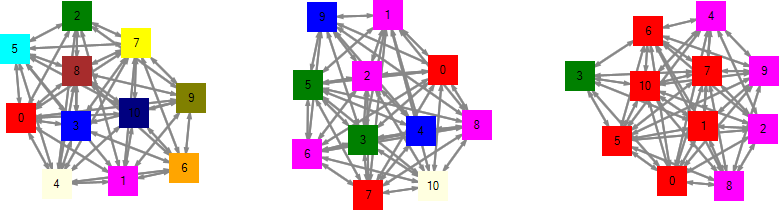
\includegraphics[width=0.5\textwidth]{abb/misc/cluster.png}
	 \caption{Eines der verwendeten Netzwerke. Die Knoten eines Cluster sind in der gleichen Farbe eingefärbt.}
	 \label{fig:cluster}
\end{figure}

\begin{figure}
	\centering
	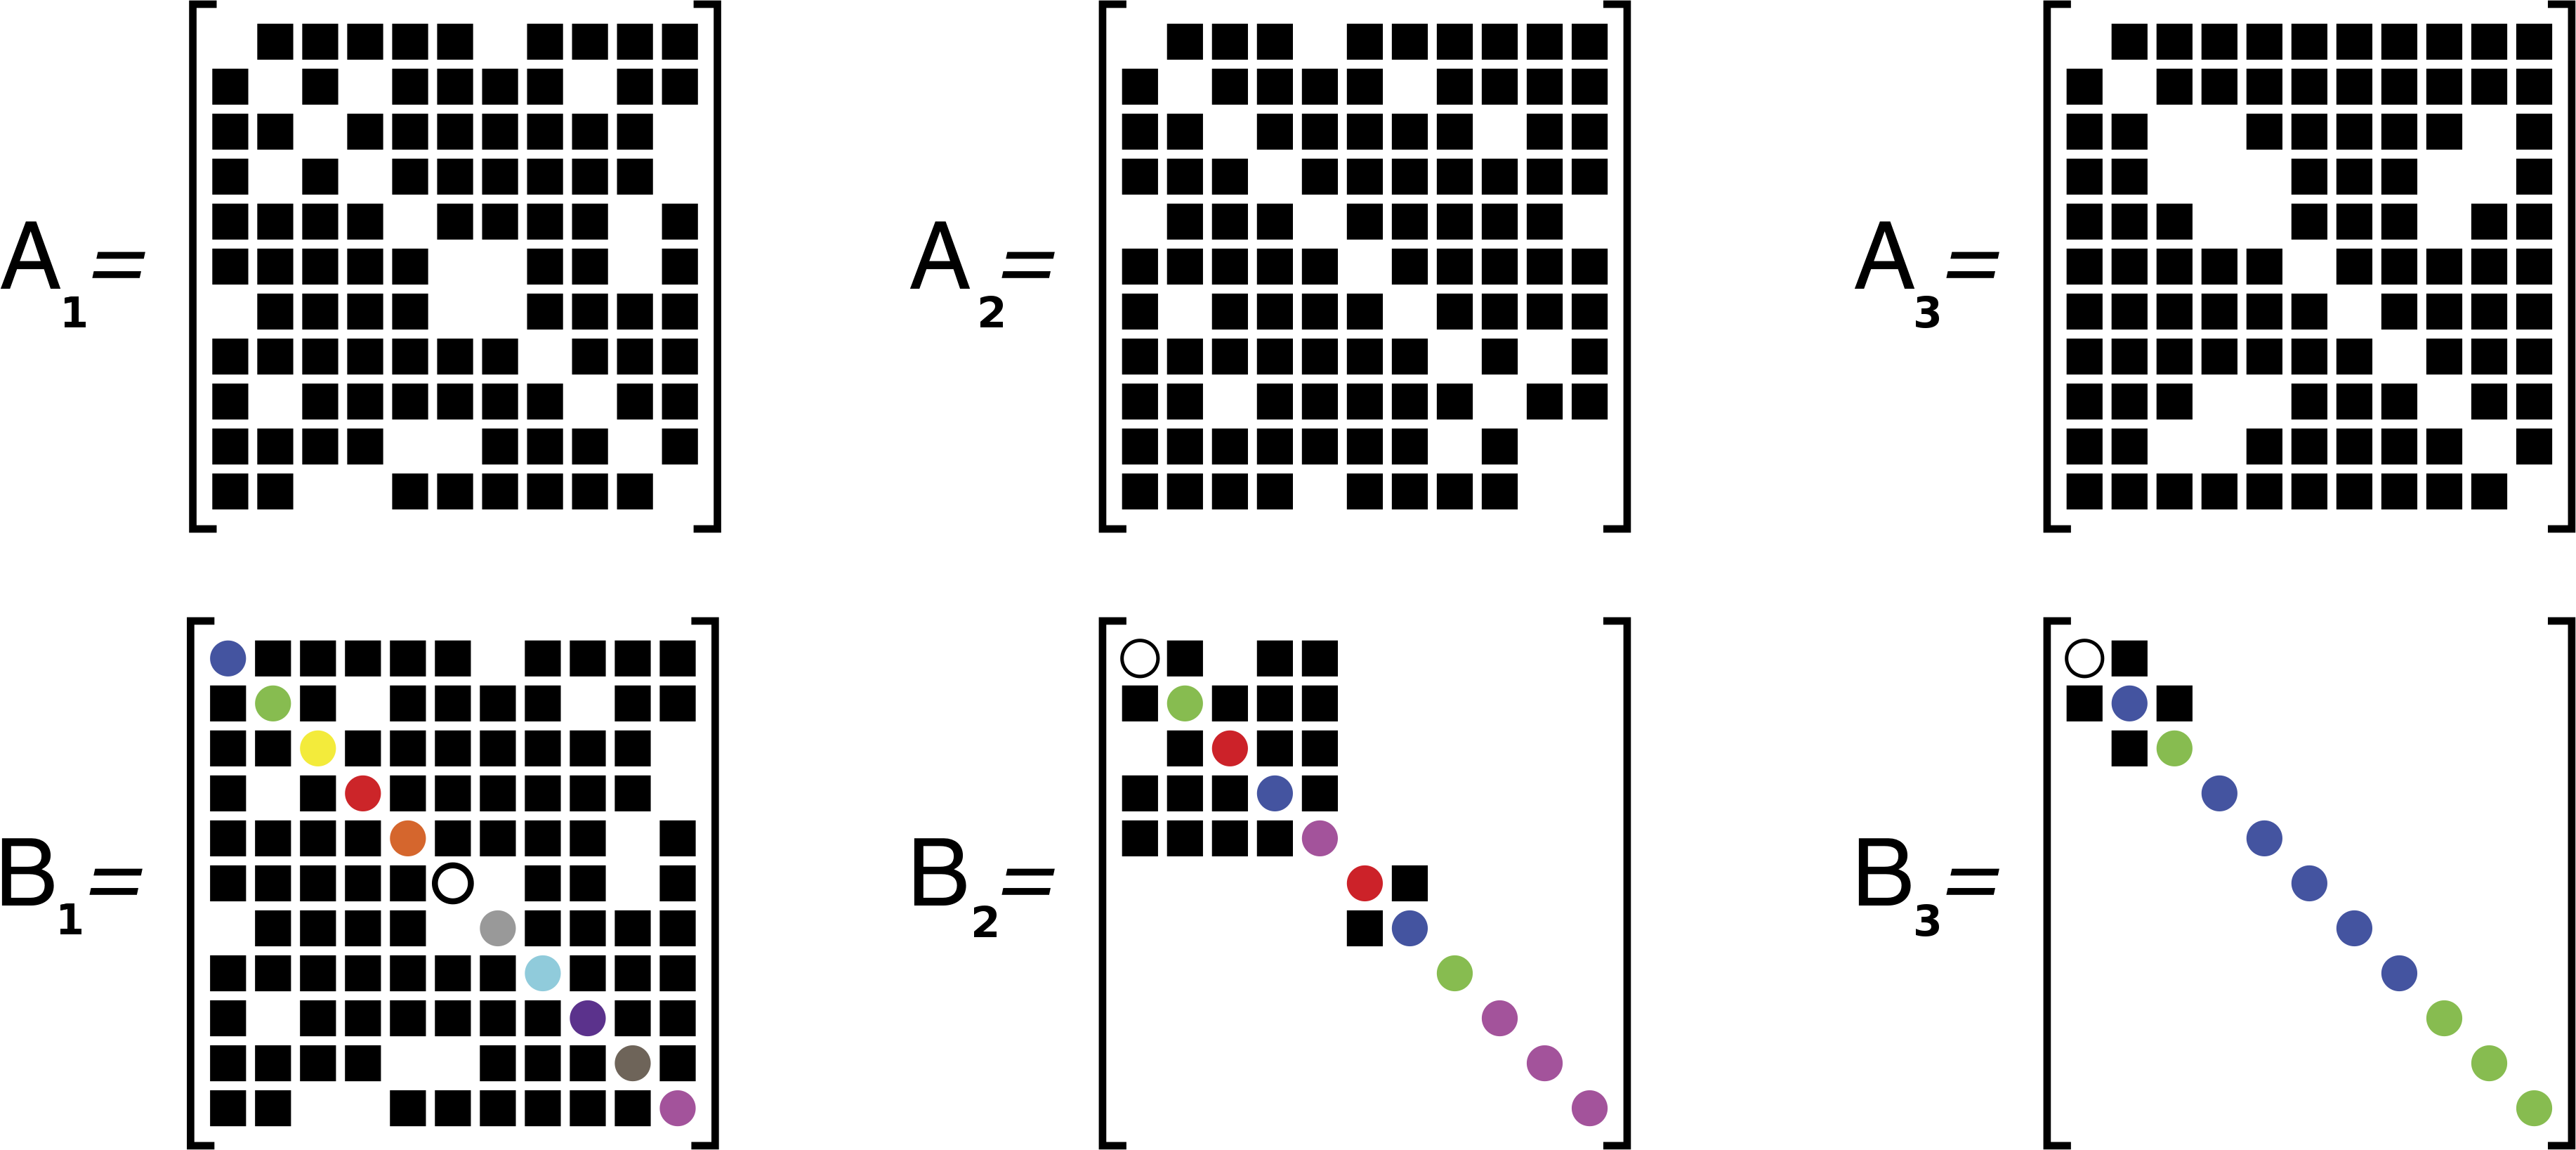
\includegraphics[width=0.5\textwidth]{abb/misc/ABMat.png}
	\caption{Kopplungsmatrix $\boldsymbol{A}$ des in Abb. \ref{fig:cluster} dargestellten Netwerks sowie die transformierte Kopplungsmatrix $\boldsymbol{B}$ in der die Zeilen nach den zugehörigen Clustern markiert sind\cite{pecora2014}.}
\label{fig:abmat}
\end{figure}

In diesen Netwerken ergibt die Clustersuche mit Nauty..


-bild vom netzwerk

-cluster, anzahl symmetrien

-rms

Zur Berechnung der Ljaponow-Exponenten wurde eine Basistransformation (siehe \ref{stabilitaet}) mit den im Anhang (\ref{Tmat}) dargestellten Transformationsmatrizen vorgenommen \cite{pecora2014,sagenotebook}
-ljapunow

